\documentclass{article}
\usepackage{minted}
\usepackage{float}
\usepackage{graphicx}
\usepackage{blindtext}
\usepackage{hyperref}
\usepackage{indentfirst}
\usepackage{amsmath}


\setlength{\parindent}{4em}
\hypersetup{
	colorlinks=true,
	linkcolor=black,
	filecolor=magenta,
	urlcolor=cyan,
	pdftitle={Overleaf Example},
	pdfpagemode=FullScreen,
}



\title{Lucrare de atestat la informatica}
\author{Matei Adriel \and Profesor Tiberiu Koos}


\begin {document}
\maketitle


\newpage
% \pagenumbering{roman}
\tableofcontents


\newpage
\section{Introducere}
\section{Motivatii}
Sistemele de tipuri sunt una dintre cele mai interesante si complexe parti ale compilatoarelor moderne.
Deducerea tipurilor incepe incet-incet sa nu mai fie doar un subiect discutat in cercetare, ci o necesitate pentru orice limaj de programare ce spera sa fie folosit in industrie.
Sistemele de tipuri pot fi implementate in multe moduri diferite, fiecare cu avatajele si dezavatajele lui.
Eu consider ca pentru a putea zice ca "intelegi" un concept din programare cu adevarat, este necesar sa poti sa il implementezi tu insusi.
La inceputul lui 2020, mi-am inceput asadar aventurile in lumea programarii functionale si a sistemelor de tipuri.

\begin{figure}[h]
	\centering
	\begin{minipage}{100px}
		\begin{minted}{c++}
auto a = 2 + 3;
\end{minted}
	\end{minipage}
	\caption{Deducerea tipului unei variabile in C++}
\end{figure}


\section{Scurta descriere}
Aplicatia lunarbox prezinta un mediu vizual pentru programarea functionala.
Toate tipurile sunt verificate, asa ca utilizatorul primeste feedback in timp real cu privire la validitatea programului sau.
In plus, numele de tiprui (ex: Int, String...) pot aparea putin ciudate pentru incepatori, asa ca fiecare dintre ele este reprezentat vizual prin o culare diferita.
Pentru a ajuta persoanele ce vor sa invete programarea functionala, lunarbox ofera 3 moduri de operare.

\newpage
\subsection{Proiecte}
Sectiunea Projects opereaza ca un sandbox, in care utilizatorul poate sa experimenteze cu orice nod oferit de lunarbox.

\begin{figure}[h]
	\centering
	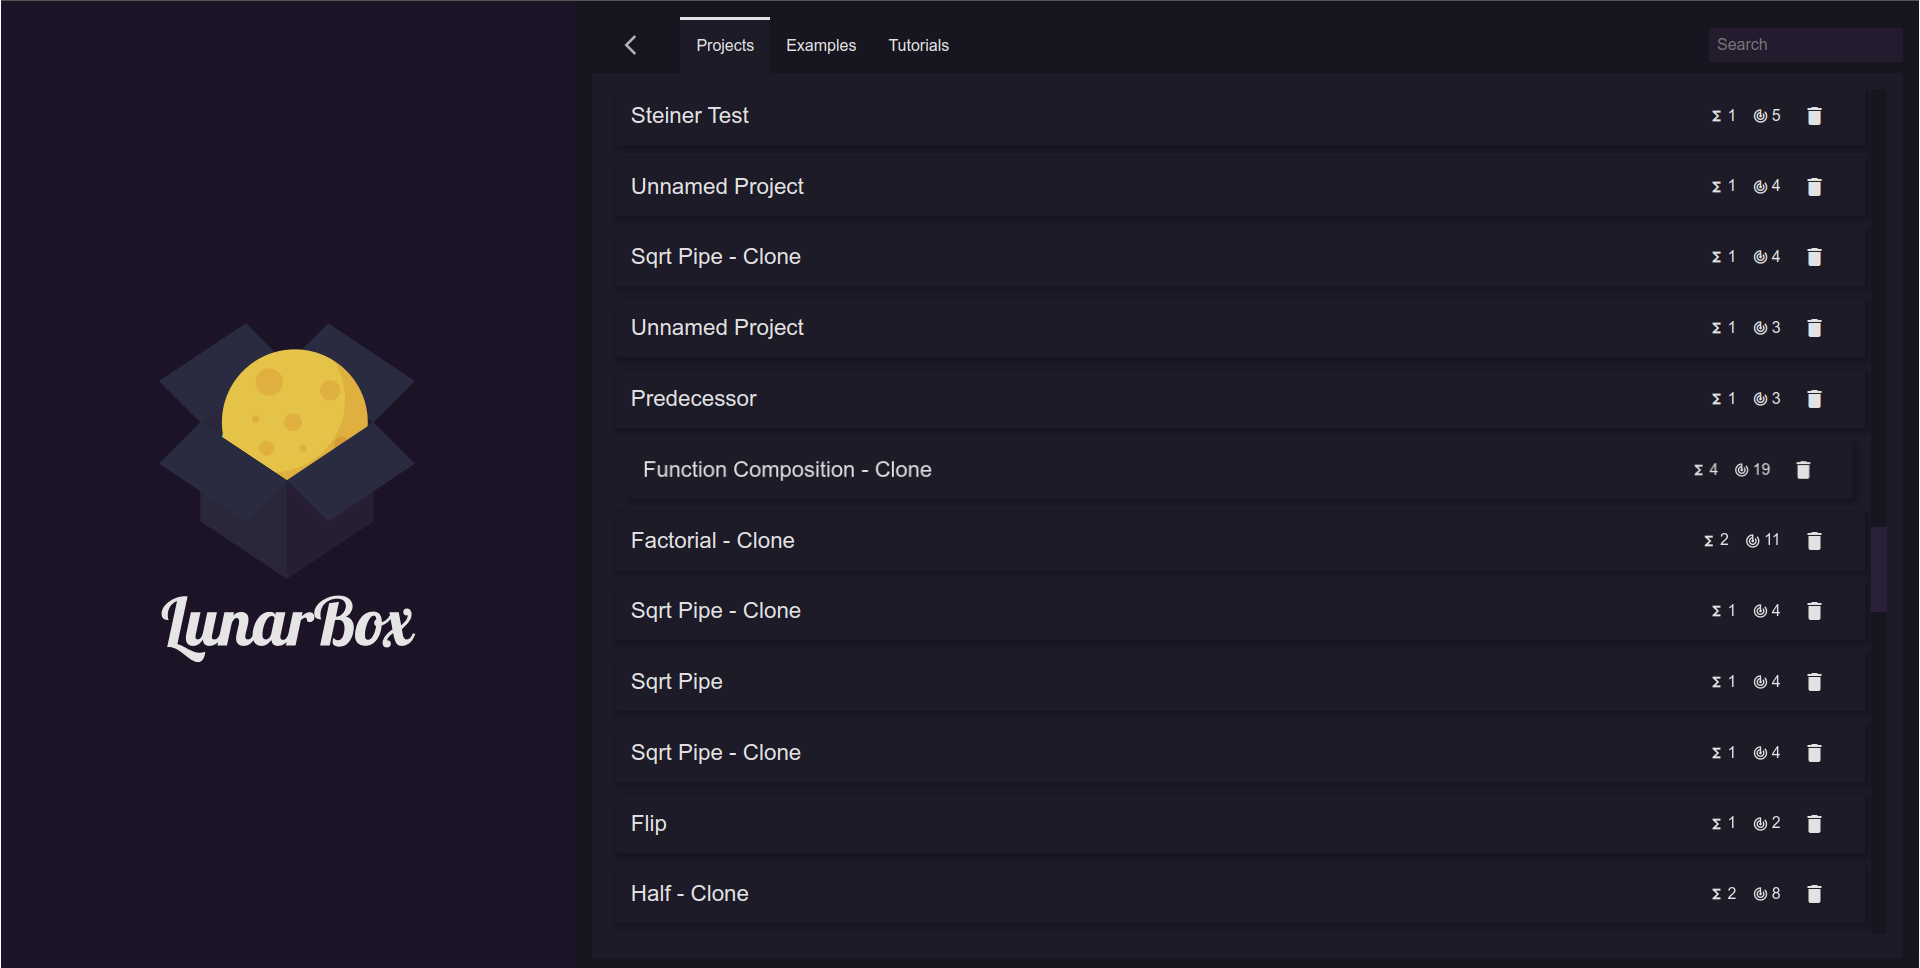
\includegraphics[width=300px]{projects.png}
	\caption{Exemplu de pagina cu proiecte al unui utilizator}
\end{figure}

\subsection{Exemple}
Sectiunea Exemple contine o serie de programe create si mentinute de adminii lunarbox.
Orice utilizator poate sa creeze o copie locala a oricarui exemplu cu un simplu click, lucru ce incurajeaza experimentarea.

\begin{figure}[h]
	\centering
	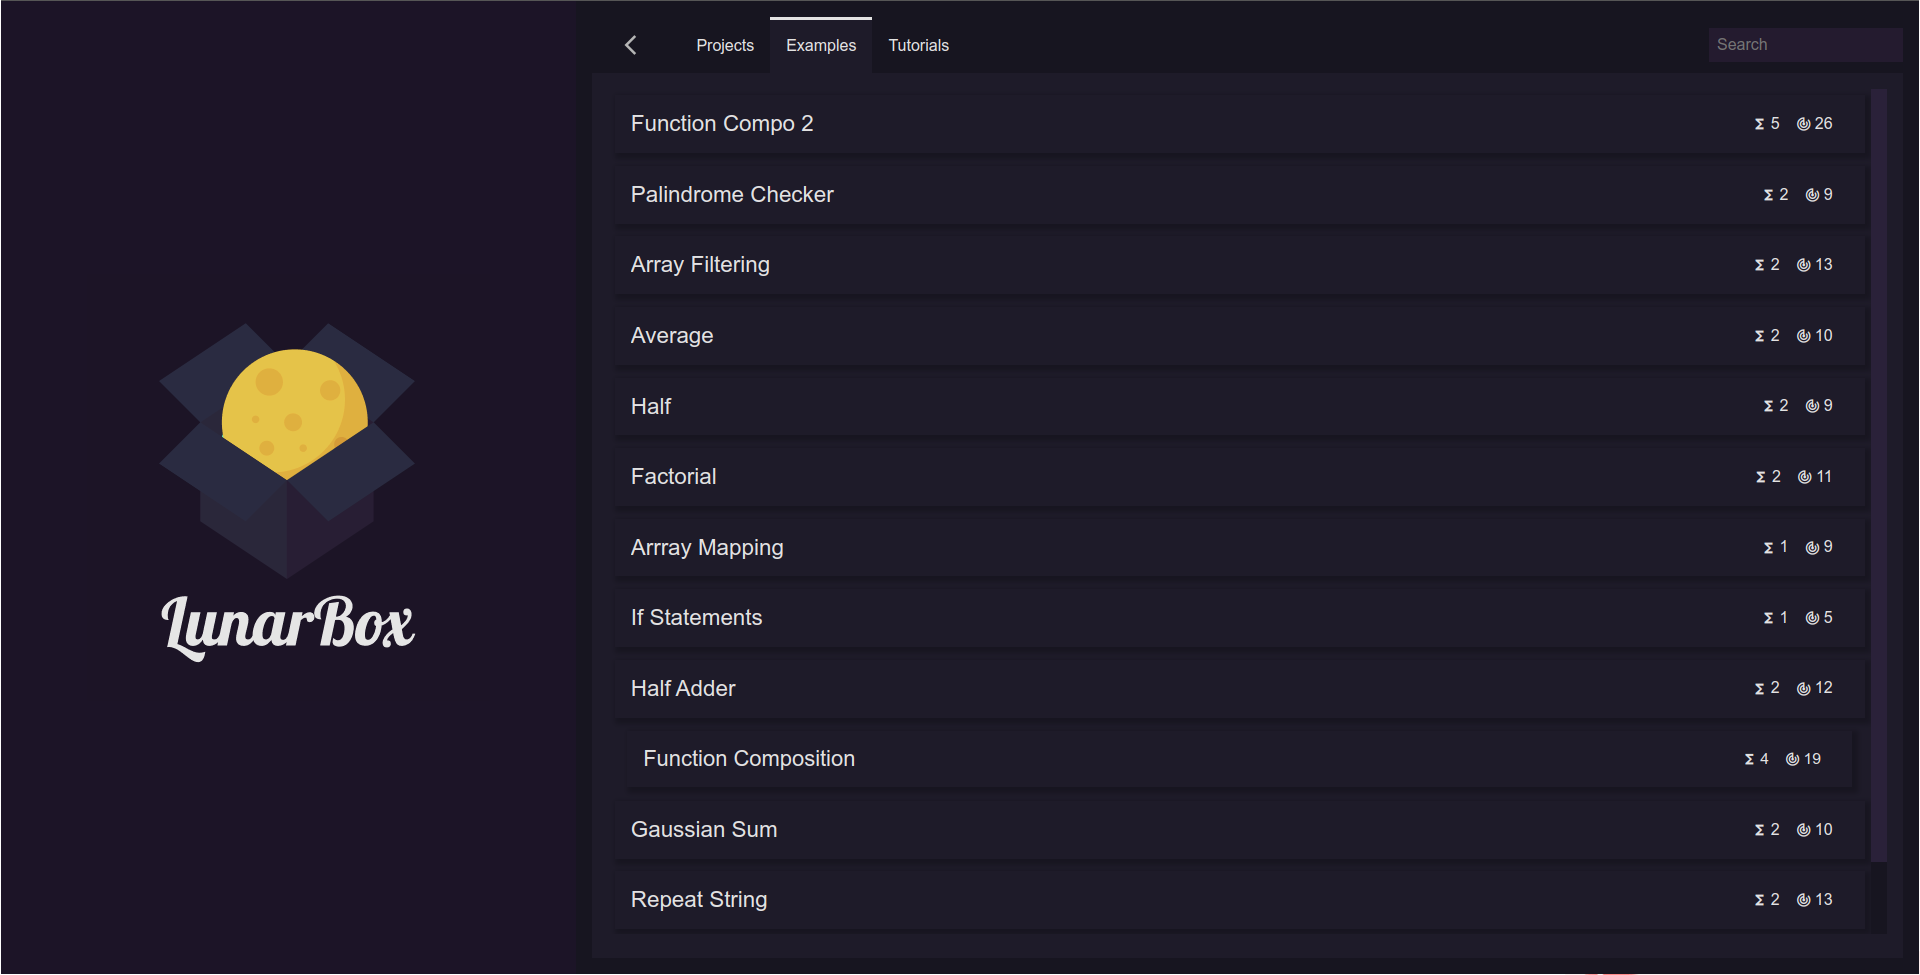
\includegraphics[width=300px]{examples.png}
	\caption{Meniul cu exemple}
\end{figure}

\subsection{Tutoriale}
Fiecare tutorial incepe cu o serie de "slide"-uri, care explica conceptul despre care este vorba.
Multe dintre slideuri contin animatii, iar utilizatorul poate chiar apasa pe unele dintre imagini pentru a deschide exemplul respectiv intr-un sandbox.
Utilizatorul este apoi confruntat cu un exercitiu.
Solutia propusa de utilizator este verificata contra unei serii de teste (similar cu siteuri precum pbinfo), iar daca raspunsul este corect, tutorialul este considerat complet.
Utilizatorul are apoi posibilitatea sa continue sa se joace cu tutorialul curent, sau sa treaca la urmatorul.
Tutorialele sunt create si intretiunte de adminii lunarbox.

\begin{figure}[h]
	\centering
	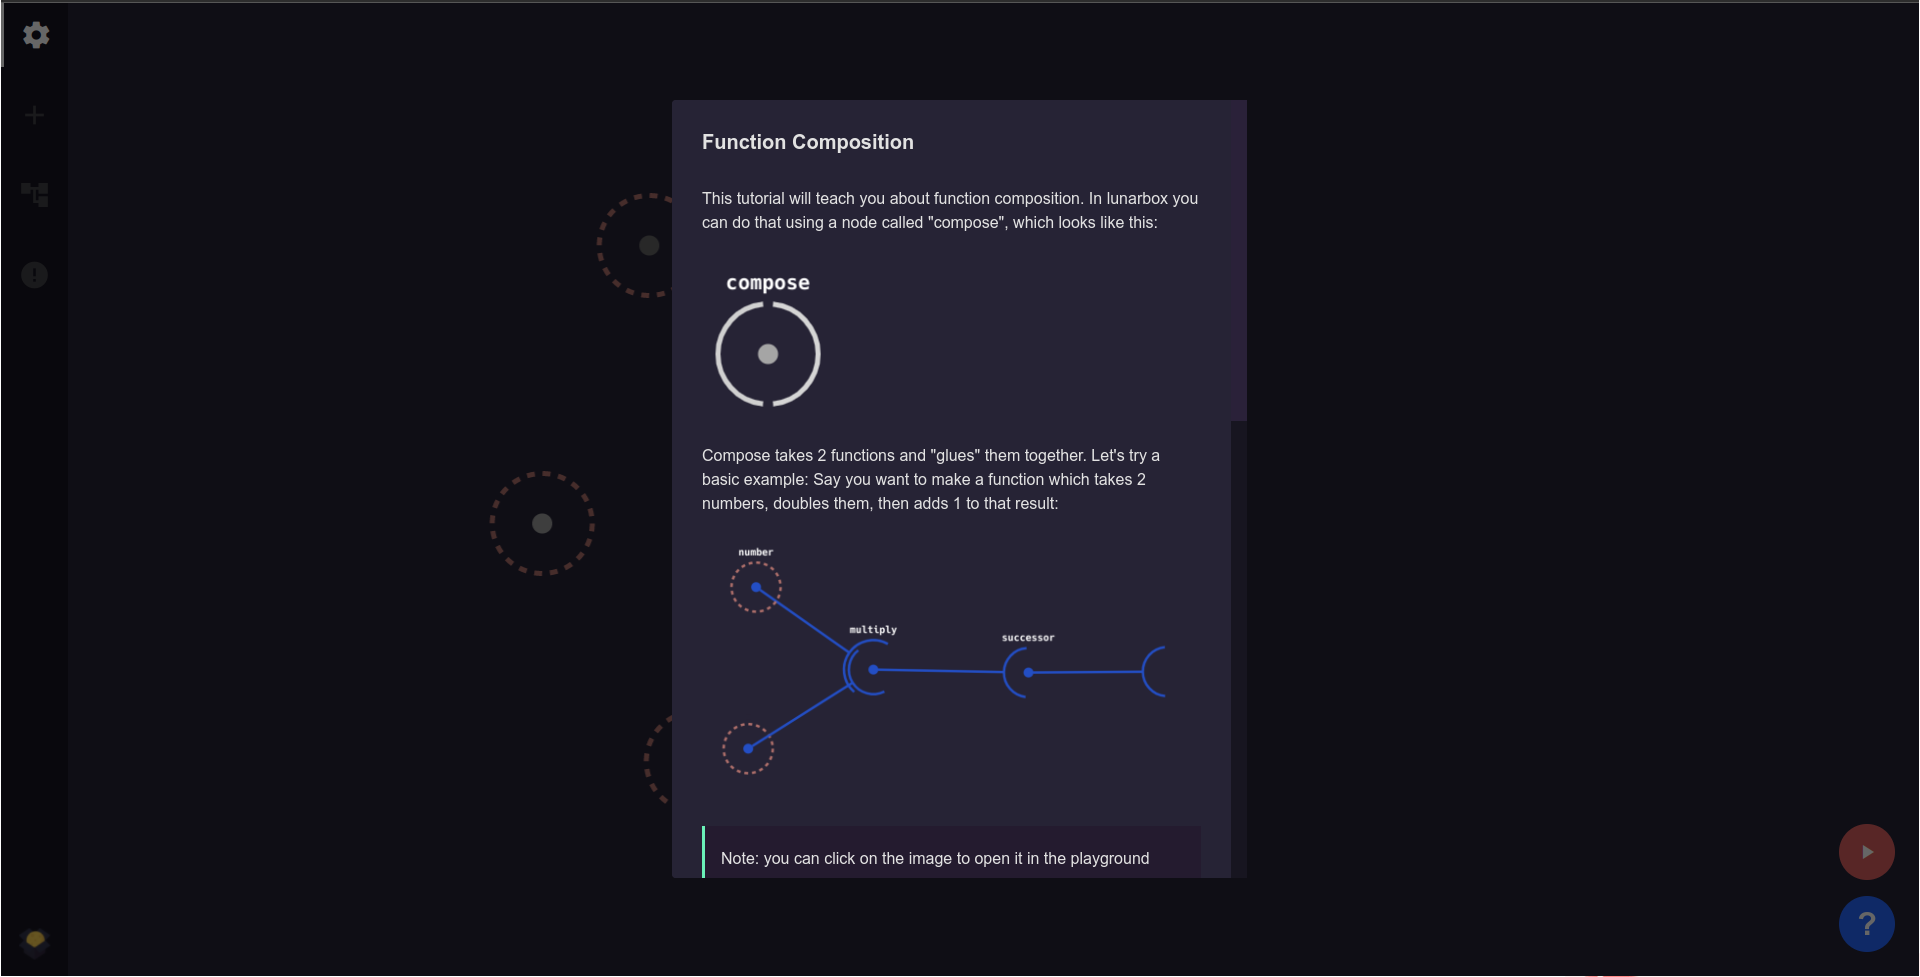
\includegraphics[width=300px]{tutorial.png}
	\caption{Tutorial-ul despre compunerea functiilor}
\end{figure}

\section{Cerinte hardware si software}
Lunarbox ruleaza pe orice calculator cu un broswer modern instalat si o conexiune la internet

\section{Descrierea aplicatiei}
Proiectul este scris intr-o combinatie dintre limbajele PureScript si TypeScript.
Doar contributia mea la proiect depaseste bariera de 10 mii de linii de cod, asa ca nu ar fi practic sa prezint toata sursa aici.
Sursa completa poate fi citita \href{https://github.com/lunarcast/lunarbox}{pe pagina de github}.

\subsection{Deducerea tipurilor}
Deducerea tipurilor este un proces relativ complex.
Am ales sa folosesc un sistem de tipuri Hindley–Milner. Functia principala pentru deducerea tipurilor, implementata in PureScript, este atasata in figura \ref{fig:infer}

\subsection{Creerea nodurilor}
Una dintre cele mai importante probleme aparute in dezvoltarea acestui proiect a fost creerea unui mod generic de a "impacheta" functii deja existene in noduri ce pot fi folosite in editorul lunarbox.
Acest lucru este mai complex decat pare - spre exemplu, sistemul de tipuri al editorului trebuie sa stie cum sa reactioneze la astfel de noduri.
Nu as avea loc pentru a arata toate fisierele ce au de aface cu aceasta problema aici.
In figura \ref{fig:typeable} se poate observa implementarea unei clase care primeste ca input un tip PureScript si returneaza un tip lunarbox.

\subsection{Interpretarea programelor}
La prima vedere, interpretarea programelor este o problema triviala (comparativ cu alte module cum ar fi sistemul de tipuri). Singurul loc unde acest lucru devine complicat este rularea functiilor recursive. Utilizatorul este liber sa defineasca astfel de functii, iar interpretatorul trebuie sa stie cum sa le execute. In figura \ref{fig:eval} am atasat codul pentru evaluarea unei expresii lunarbox


\begin{figure}[ht]
	\centering
	\begin{minted}{haskell}
-- Infers a type and marks it's location on the typeMap
infer :: forall l. Ord l => Show l => Expression l -> Infer l Type
infer expression =
  withLocation (getLocation expression) do
    type' <- case expression of
      Variable _ name -> do
        lookupEnv name
      Lambda _ param body -> do
        tv <- fresh true
        t <- createClosure param (Forall [] tv) $ infer body
        pure $ typeFunction tv t
      FunctionCall _ func input -> do
        funcType <- infer func
        inputType <- infer input
        tv <- fresh true
        createConstraint funcType (typeFunction inputType tv)
        pure tv
      If _ cond then' else' -> do
        tyCond <- infer cond
        tyThen <- infer then'
        tyElse <- infer else'
        tv <- fresh true
        createConstraint tyCond typeBool
        createConstraint tv tyThen
        createConstraint tv tyElse
        pure tv
      Let location name value body -> do
        env <- ask
        Tuple valueType (InferOutput { constraints }) <- listen $ infer value
        let
          (Tuple subst (SolveState { errors })) = runSolve (SolveContext { location }) $ solve constraints
        for_ errors $ createError <<< Stacked
        generalized <- local (const $ apply subst env) $ generalize $ apply subst valueType
        createClosure name generalized $ infer body
      FixPoint loc name body -> do
        tv <- fresh true
        ty <- createClosure name (Forall [] tv) $ infer body
        createConstraint tv ty
        pure ty
      Expression _ inner -> infer inner
      TypedHole _ -> fresh false
      Native _ (NativeExpression scheme _) -> instantiate scheme
    rememberType type'
\end{minted}

	\caption{Deducerea tipurilor implementata in PureScript}
	\label{fig:infer}
\end{figure}

\begin{figure}[ht]
	\centering
	\begin{minted}{haskell}
class Typeable (a :: Type) where
  typeof :: Proxy a -> Type

instance typeableNumber :: Typeable Number where
  typeof _ = typeNumber

instance typeableInt :: Typeable Int where
  typeof _ = typeNumber

instance typeableString :: Typeable String where
  typeof _ = typeString

instance typeableBool :: Typeable Boolean where
  typeof _ = typeBool

instance typeableArray :: Typeable a => Typeable (Array a) where
  typeof _ = typeArray (typeof (Proxy :: Proxy a))

instance typePair :: (Typeable a, Typeable b) => Typeable (Tuple a b) where
  typeof _ = typePair (typeof _a) (typeof _b)
    where
    _a :: Proxy a
    _a = Proxy
    
    _b :: Proxy b
    _b = Proxy

instance typeableSymbol :: IsSymbol sym => Typeable (SProxy sym) where
  typeof _ = TVariable true $ TVarName $ reflectSymbol (SProxy :: SProxy sym)

instance typeableArrow :: (Typeable a, Typeable b) => Typeable (a -> b) where
  typeof _ = typeFunction (typeof (Proxy :: Proxy a)) (typeof (Proxy :: Proxy b))

-- | Get the type of a purescript value
getType :: forall a. Typeable a => a -> Type
getType _ = typeof (Proxy :: Proxy a)
\end{minted}
	\caption{"Impachetarea" tipurilor native din PureScript ca tipuri pentru noduri din editor}
	\label{fig:typeable}
\end{figure}

\begin{figure}[ht]
	\centering
	\begin{minted}{haskell}
interpret :: forall l. Ord l => Default l => Expression l -> Interpreter l (Term l)
interpret expression = do
  overwrites <- asks $ view _overwrites
  -- ... mai multe definitii irelevante scoase pentru a aveam spatiu
  value <- case maybeOverwrite of
    Just overwrite -> pure overwrite
    Nothing -> case expression of
      TypedHole _ -> pure $ Term Null
      Variable _ name -> getVariable $ show name
      Lambda _ _ _ -> do
        env <- getEnv
        pure $ Closure env expression
      Expression _ inner -> interpret inner
      If _ cond then' else' -> interpret cond >>= go
	-- ... mai multe definitii irelevante scoase pentru a aveam spatiu
      Let _ name value body -> do
        runtimeValue <- interpret value
        withTerm (show name) runtimeValue $ interpret body
      expr@(FixPoint l name body) -> do
        env <- getEnv
        let self = Closure env expr
        withTerm (show name) self $ interpret body
      Native _ (NativeExpression _ inner) -> pure $ Term inner
      FunctionCall _ function argument -> do
        runtimeArgument <- interpret argument
        runtimeFunction <- interpret function
        let
          go = case _ of
            Closure env (Lambda _ name expr) ->
              scoped $ withEnv env $ withTerm (show name) runtimeArgument
                $ interpret expr
            Closure env expr -> call >>= go
              where
              call = scoped $ withEnv env $ interpret expr
            Term (Function call) -> do
              ctx <- ask
              pure $ Term $ call $ termToRuntime ctx runtimeArgument
            Term _ -> pure def
        go runtimeFunction
  toplevel <- asks $ view _toplevel
  when toplevel $ tell $ ValueMap $ Map.singleton location value
  pure value
\end{minted}
	\caption{Evaluarea expresiilor in lunarbox}
	\label{fig:eval}
\end{figure}

\subsection{De la grafuri la arbori ai sintaxei}
\par Majoritatea algoritmilor pentru interpretarea limbajelor de programare, sisteme de tipuri, etc, lucreaza pe arbori de sintaxa abstracta (AST).
Programele create de utilizatori in editor iau forma unui graf orientat, asa ca am creat un algoritm care sa converteasca astfel de structuri inr-un limbaj intern standard, pe care urmeaza sa rulez mai apoi restul modulelor.
Figura \ref{img:graph} exemplifica structura de graf a programelor lunarbox, iar figura \ref{fig:expr} arata AST-ul in care aceste structuri sunt transformate.

\begin{figure}[H]
	\centering
	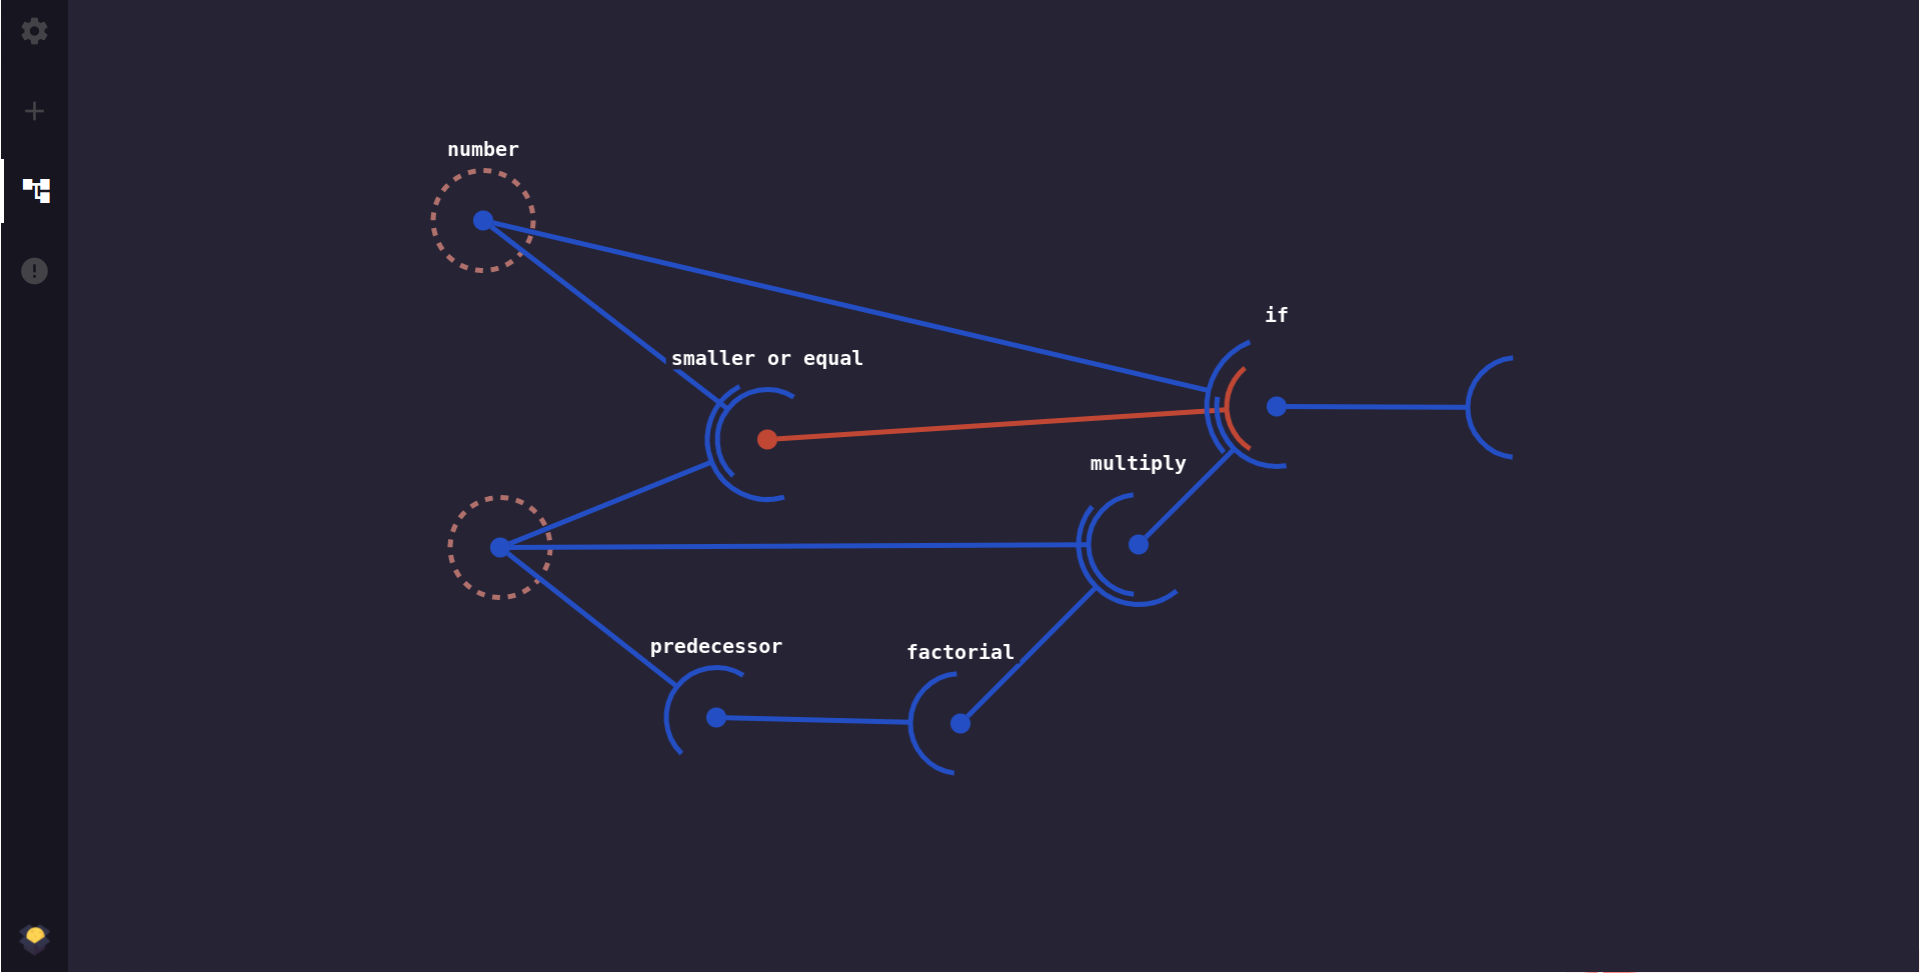
\includegraphics[width=300px]{graph.png}
	\caption{Program lunarbox ce ilustreaza structura de graf}
	\label{img:graph}
\end{figure}

\begin{figure}[H]
	\centering
	\begin{minted}{haskell}
newtype VarName
  = VarName String

data NativeExpression
  = NativeExpression Scheme RuntimeValue

data Expression l
  = Variable l VarName
  | FunctionCall l (Expression l) (Expression l)
  | Lambda l VarName (Expression l)
  | Let l VarName (Expression l) (Expression l)
  | If l (Expression l) (Expression l) (Expression l)
  | FixPoint l VarName (Expression l)
  | Expression l (Expression l)
  | Native l NativeExpression
  | TypedHole l
\end{minted}
	\caption{Tipul de date pentru AST-ul lunarbox}
	\label{fig:expr}
\end{figure}


\section{Concluzii}
\subsection{Monazii - o solutie eleganta pentru lucrul cu efecte}
Cand zic efecte, nu ma refer la sensul colocvial al cuvantului, ci la cel din domeniul programarii functionale.
Un efect este o actiune ce nu e pura (ex: afisarea unei propozitii pe ecran).
Codul din figura \ref{fig:infer} foloseste multe astfel de efecte (generarea de id-uri unice, colectarea de "constrangeri", memorarea rezultatelor intermediare, indexarea unui "context", etc), toate aceste efecte fiind atat verificate de sistemul de tiprui al limbajului PureScript cat si suficient de "ne-intrusive" incat codul arata ca si cum ar fi scris intr-un DSL (domain-specific-language) special facut pentru aceasta problema.
Consider ca monazii sunt o solutie excelenta pentru astfel de probleme.

\subsection{Programarea functionala ca metoda de implementare a sistemelor complexe}
\par Imi doresc ca acest proiect sa fie o dovada vie ca limbajele de programare precum PureScript (care la randul sau este foarte similar cu Haskell) sunt o solutie excelenta pentru creerea si intretinerea de sisteme ce prezinta complexitate ridicata.
\par
Proiectul meu contine multe alte module pe care nu le-asi fi putut prezenta fara a ocupa foarte mult spatiu (un sistem de conturi, optiuni pentru admini, un sistem de "warninguri" si un optimizator pentru AST-ul lunarbox, etc).
Paradigma programarii functionale este o solutie excelenta pentru astfel de proiecte, deoarece folosita corect poate duce la programe usor de extins si intretinut.

\section{Limits}
\subsection{Definition}
\par
\begin{equation*} \label{Limit definition}
	\begin{aligned}
		\lim_{x \to \alpha} f(x) = L & \iff
		\\\forall \epsilon&, \epsilon > 0 \to
		\\\exists \sigma&,  \sigma > 0,
		\\\forall x&, 0 < |x - a| < \sigma \to
		|f(x) - L| < \epsilon
	\end{aligned}
\end{equation*}
\subsection{Using neighbourhoods}
\par
\begin{equation*} \label{Limit definition using neighbourhoods}
	\begin{aligned}
		\lim_{x \to \alpha} f(x) & = L \iff
		\\\forall \epsilon &, \epsilon > 0 \to
		\\\exists \sigma &, \sigma > 0,
		\\\forall x &, x \in I_{0}(a, \sigma) \to
		f(x) \in I(L, \epsilon)
	\end{aligned}
\end{equation*}

% \begin{figure}[ht]
% \begin{minted}{javascript}
% async function() {
%   const foo = await operation1()
%   const bar = await operation2()
% 
%   return foo + bar;
% }
% 
% \end{minted}
% \end{figure}

\end {document}


